% coding:utf-8

%FOSAET, a LaTeX-Code for a electrical summary of basic electronics
%Copyright (C) 2013, Daniel Winz, Ervin Mazlagic

%This program is free software; you can redistribute it and/or
%modify it under the terms of the GNU General Public License
%as published by the Free Software Foundation; either version 2
%of the License, or (at your option) any later version.

%This program is distributed in the hope that it will be useful,
%but WITHOUT ANY WARRANTY; without even the implied warranty of
%MERCHANTABILITY or FITNESS FOR A PARTICULAR PURPOSE.  See the
%GNU General Public License for more details.
%----------------------------------------

% coding:utf-8

%FOSAET, a LaTeX-Code for a electrical summary of basic electronics
%Copyright (C) 2013, Daniel Winz, Ervin Mazlagic

%This program is free software; you can redistribute it and/or
%modify it under the terms of the GNU General Public License
%as published by the Free Software Foundation; either version 2
%of the License, or (at your option) any later version.

%This program is distributed in the hope that it will be useful,
%but WITHOUT ANY WARRANTY; without even the implied warranty of
%MERCHANTABILITY or FITNESS FOR A PARTICULAR PURPOSE.  See the
%GNU General Public License for more details.
%----------------------------------------

\section{Zählpfeilsysteme}

\begin{figure}[h!]
	\centering
	\begin{subfigure}[b]{0.4\textwidth}
		\centering
		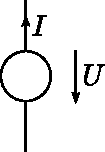
\includegraphics[scale=\schscale]{erzpfeilsys_sch.pdf}
		\caption{Erzeugerpfeilsystem}
		\label{sch:erzpfeilsys}
	\end{subfigure}
	\begin{subfigure}[b]{0.4\textwidth}
		\centering
		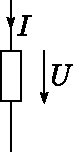
\includegraphics[scale=\schscale]{verbpfeilsys_sch.pdf}
		\caption{Verbraucherpfeilsystem}
		\label{sch:verbpfeilsys}
	\end{subfigure}
	\caption{Zählpfeilsysteme}
	\label{sch:pfeilsys}
\end{figure}

\subsection{Erzeugerpfeilsystem}
Zweipol wirk als Erzeuger, wenn das Produkt aus $U$ und $I$ positiv ist. Sonst wirkt er als Verbraucher. 

\subsection{Verbraucherpfeilsystem}
Zweipol wirk als Verbraucher, wenn das Produkt aus $U$ und $I$ positiv ist. Sonst wirkt er als Erzeuger. 
    % Pfeilsysteme
% coding:utf-8

%FOSAET, a LaTeX-Code for a electrical summary of basic electronics
%Copyright (C) 2013, Daniel Winz, Ervin Mazlagic

%This program is free software; you can redistribute it and/or
%modify it under the terms of the GNU General Public License
%as published by the Free Software Foundation; either version 2
%of the License, or (at your option) any later version.

%This program is distributed in the hope that it will be useful,
%but WITHOUT ANY WARRANTY; without even the implied warranty of
%MERCHANTABILITY or FITNESS FOR A PARTICULAR PURPOSE.  See the
%GNU General Public License for more details.
%----------------------------------------

\section{Ohmsches Gesetz}
\noindent
\[ \begin{array}{l}
U = R \cdot I\\\\
I = \frac{U}{R}\\\\
R = \frac{U}{I}
\end{array}\]
\begin{tabular}{lll}
\multicolumn{2}{l}{Variable}&Einheit\\\\
$U$&Spannung&Volt $[V]$\\\\
$I$&Strom&Ampere $[A]$\\\\
$R$&Widerstand&Ohm $[\Omega]$
\end{tabular}         % Ohmsches Gesetz
% coding:utf-8

%FOSAET, a LaTeX-Code for a electrical summary of basic electronics
%Copyright (C) 2013, Daniel Winz, Ervin Mazlagic

%This program is free software; you can redistribute it and/or
%modify it under the terms of the GNU General Public License
%as published by the Free Software Foundation; either version 2
%of the License, or (at your option) any later version.

%This program is distributed in the hope that it will be useful,
%but WITHOUT ANY WARRANTY; without even the implied warranty of
%MERCHANTABILITY or FITNESS FOR A PARTICULAR PURPOSE.  See the
%GNU General Public License for more details.
%----------------------------------------

\section{Leistung}
\[ P = U \cdot I = \frac{U^2}{R} = I^2 \cdot R \]       % Leistung
% coding:utf-8

%FOSAET, a LaTeX-Code for a electrical summary of basic electronics
%Copyright (C) 2013, Daniel Winz, Ervin Mazlagic

%This program is free software; you can redistribute it and/or
%modify it under the terms of the GNU General Public License
%as published by the Free Software Foundation; either version 2
%of the License, or (at your option) any later version.

%This program is distributed in the hope that it will be useful,
%but WITHOUT ANY WARRANTY; without even the implied warranty of
%MERCHANTABILITY or FITNESS FOR A PARTICULAR PURPOSE.  See the
%GNU General Public License for more details.
%----------------------------------------

\section{Kirchhoffsche Gesetze}

\subsection{Maschenregel}
Die Spannung in einer geschlossenen Masche ist 0. 
\[ \sum U = 0 \]

\subsection{Knotenregel}
Alle Ströme, die in einen Knoten hineinfliessen ergeben in der Summe 0. 
\[ \sum I = 0 \]

\subsection{Super-Knoten}
Die Kirchhoff'sche Knotenregel besagt, dass die Summe aller Ströme eines Knoten gleich Null ist.
Dieser Zusammenhang kann auch dann genutzt werden wenn keine idealen Knoten vorhanden sind.
Eine Schaltung kann beliebig zu einen Knoten abstrahiert werden und die Knotenströme zu ermitteln.

\begin{figure}[h!]
\centering
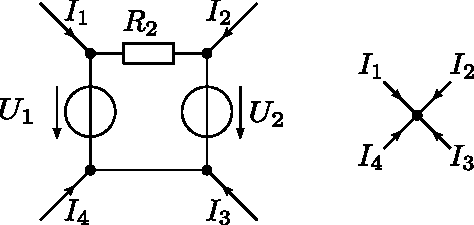
\includegraphics[scale=\schscale]{supernode_sch.pdf}
\caption{Super-Knoten}
\label{sch:supernode}
\end{figure}

\noindent
\textbf{Achtung!} Dieses Prinzip der Zusammenfassung einer Schaltung zu einem Knoten darf nur dazu genutzt werden, um die Ströme in und aus dem Knoten heraus zu ermitteln. Die abstrahierte Schaltung in innern darf jedoch nicht ohne diese Ströme betrachtet werden. 
       % Kirchhoffsche Gesetze
% coding:utf-8

%FOSAET, a LaTeX-Code for a electrical summary of basic electronics
%Copyright (C) 2013, Daniel Winz, Ervin Mazlagic

%This program is free software; you can redistribute it and/or
%modify it under the terms of the GNU General Public License
%as published by the Free Software Foundation; either version 2
%of the License, or (at your option) any later version.

%This program is distributed in the hope that it will be useful,
%but WITHOUT ANY WARRANTY; without even the implied warranty of
%MERCHANTABILITY or FITNESS FOR A PARTICULAR PURPOSE.  See the
%GNU General Public License for more details.
%----------------------------------------

\section{Spannungsteiler}

\subsection{unbelasteter Spannungsteiler}
\begin{figure}[h!]
	\centering
	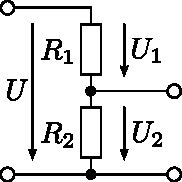
\includegraphics[scale=\schscale]{uteil.pdf}
	\caption{unbelasteter Spannungsteiler}
	\label{sch:uteil}
\end{figure}
\[ U_2 = \frac{U_1}{R_1 + R_2} \cdot R_2 \]

\subsection{belasteter Spannungsteiler}
\begin{figure}[h!]
	\centering
	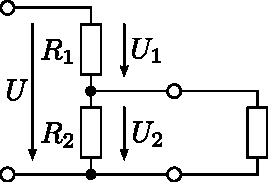
\includegraphics[scale=\schscale]{uteilbel.pdf}
	\caption{belasteter Spannungsteiler}
	\label{sch:uteilbel}
\end{figure}
\[ U_2 = \frac{U_1}{R_1 + \frac{R_2 \cdot R_L}{R_2 + R_L}} \cdot \frac{R_2 \cdot R_L}{R_2 + R_L} \]

\subsection{unbelastetes Potentiometer}
\[ U_2 = U_1 \cdot \ell \]

\subsection{belastetes Potentiometer}
\[ U_2 = \frac{U_1}{R_p \cdot (1 - \ell) + \frac{R_p \cdot \ell \cdot R_L}{R_p \cdot \ell + R_L}} \cdot \frac{R_p \cdot \ell \cdot R_L}{R_p \cdot \ell + R_L} \]
       % Spannungsteiler
% coding:utf-8

%----------------------------------------
%FOSAMATH, a LaTeX-Code for a mathematical summary for basic analysis
%Copyright (C) 2013, Daniel Winz, Ervin Mazlagic, Adrian Imboden, Philipp Langer

%This program is free software; you can redistribute it and/or
%modify it under the terms of the GNU General Public License
%as published by the Free Software Foundation; either version 2
%of the License, or (at your option) any later version.

%This program is distributed in the hope that it will be useful,
%but WITHOUT ANY WARRANTY; without even the implied warranty of
%MERCHANTABILITY or FITNESS FOR A PARTICULAR PURPOSE.  See the
%GNU General Public License for more details.
%----------------------------------------

% coding:utf-8
\section{Stromteiler}       % Stromteiler
% coding:utf-8

%----------------------------------------
%FOSAMATH, a LaTeX-Code for a mathematical summary for basic analysis
%Copyright (C) 2013, Daniel Winz, Ervin Mazlagic, Adrian Imboden, Philipp Langer

%This program is free software; you can redistribute it and/or
%modify it under the terms of the GNU General Public License
%as published by the Free Software Foundation; either version 2
%of the License, or (at your option) any later version.

%This program is distributed in the hope that it will be useful,
%but WITHOUT ANY WARRANTY; without even the implied warranty of
%MERCHANTABILITY or FITNESS FOR A PARTICULAR PURPOSE.  See the
%GNU General Public License for more details.
%----------------------------------------

% coding:utf-8
\section{Spezifisscher Widerstand}     % Spezifischer Widerstand
% coding:utf-8

%FOSAET, a LaTeX-Code for a electrical summary of basic electronics
%Copyright (C) 2013, Daniel Winz, Ervin Mazlagic

%This program is free software; you can redistribute it and/or
%modify it under the terms of the GNU General Public License
%as published by the Free Software Foundation; either version 2
%of the License, or (at your option) any later version.

%This program is distributed in the hope that it will be useful,
%but WITHOUT ANY WARRANTY; without even the implied warranty of
%MERCHANTABILITY or FITNESS FOR A PARTICULAR PURPOSE.  See the
%GNU General Public License for more details.
%----------------------------------------

\section{Temperaturabhäigkeit von Widerständen}

\subsection{Lineare Temperaturabhängigkeit von Widerständen}
\[ R_\vartheta = R_{20} \cdot (1 + \alpha \cdot \Delta \vartheta \]
\[ \Delta R = R_{20} \cdot \alpha \cdot \Delta \vartheta \]
Falls $R_{20}$ nicht bekannt ist, kann mit $R_A$ bei $\vartheta_a$ und $\tau$ die Temperaturabhängigkeit mit folgender Formel berechnet werden:  \[ R_\vartheta = R_A \frac{\tau + \vartheta}{\tau + \vartheta_A} \]
Wobei 
\[ \tau = \frac{1}{\alpha_20} - 20^{\circ}\text{C} \]

\subsection{Nichtlineare Temperaturabhängigkeit (PTC)}
\[ R_T = R_N \cdot e^{\alpha (T - T_N)} \]
\[ \alpha = \frac{\ln R_2 - \ln R_1}{T_2 - T_1} = \frac{d R_t}{d T}\frac{1}{R_T} \]

\subsection{Nichtlineare Temperaturabhängigkeit (NTC)}
\[ R_T = R_N \cdot e^{b\left(\frac{1}{T} - \frac{1}{T_N}\right)} \]
\[ \alpha_T = \frac{d R_T}{d T}\frac{1}{R_T} = -\frac{b}{T^2} \]     % Temperaturabhängigkeit von Widerständen
% coding:utf-8

%----------------------------------------
%FOSAMATH, a LaTeX-Code for a mathematical summary for basic analysis
%Copyright (C) 2013, Daniel Winz, Ervin Mazlagic, Adrian Imboden, Philipp Langer

%This program is free software; you can redistribute it and/or
%modify it under the terms of the GNU General Public License
%as published by the Free Software Foundation; either version 2
%of the License, or (at your option) any later version.

%This program is distributed in the hope that it will be useful,
%but WITHOUT ANY WARRANTY; without even the implied warranty of
%MERCHANTABILITY or FITNESS FOR A PARTICULAR PURPOSE.  See the
%GNU General Public License for more details.
%----------------------------------------

% coding:utf-8
\section{Brückenschaltung}      % Brückenschaltung
% coding:utf-8

%FOSAET, a LaTeX-Code for a electrical summary of basic electronics
%Copyright (C) 2013, Daniel Winz, Ervin Mazlagic

%This program is free software; you can redistribute it and/or
%modify it under the terms of the GNU General Public License
%as published by the Free Software Foundation; either version 2
%of the License, or (at your option) any later version.

%This program is distributed in the hope that it will be useful,
%but WITHOUT ANY WARRANTY; without even the implied warranty of
%MERCHANTABILITY or FITNESS FOR A PARTICULAR PURPOSE.  See the
%GNU General Public License for more details.
%----------------------------------------

\section{Leistungsanpassung}      % Leistungsanpassung
% coding:utf-8

%----------------------------------------
%FOSAMATH, a LaTeX-Code for a mathematical summary for basic analysis
%Copyright (C) 2013, Daniel Winz, Ervin Mazlagic, Adrian Imboden, Philipp Langer

%This program is free software; you can redistribute it and/or
%modify it under the terms of the GNU General Public License
%as published by the Free Software Foundation; either version 2
%of the License, or (at your option) any later version.

%This program is distributed in the hope that it will be useful,
%but WITHOUT ANY WARRANTY; without even the implied warranty of
%MERCHANTABILITY or FITNESS FOR A PARTICULAR PURPOSE.  See the
%GNU General Public License for more details.
%----------------------------------------

% coding:utf-8
\section{Umwandlung Spannungsquelle $\leftrightarrow$ Stromquelle}

\subsection{Thévenin-Theorem}
Nach Thévenin kann jedes Netzwerk bestehend aus Strom-, Spannungsquellen und Widerständen in eine Ersatzspannungsquelle\footnote{Thévenin-Äquivalent} gewandelt werden.

\begin{figure}[h!]
\centering
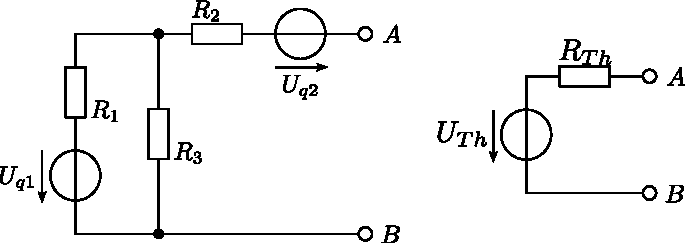
\includegraphics[scale=\schscale]{thevenin_sch_2.pdf}
\label{sch:thevenin}
\caption{Schaltung (l) und ihr Thévenin-Äquivalent (r)}
\end{figure}

\subsubsection{Berechnung}
\begin{itemize}
\item Leerlaufspannung $U_{Th}$ bestimmen (siehe Kapitel~\ref{sec:superpos})
\item Ersatzwiderstand ermitteln durch ausschalten aller unabhängiger Quellen (Spannungsquellen werden kurzgeschlossen, Stromquellen unterbrochen)
\end{itemize}

\subsection{Norton-Theorem}
Nach Norton kann jedes Netzwerk bestehend aus Strom-, Spannungsquellen und Widerständen in eine Ersatzstromquelle\footnote{Norton-Äqivalent} gewandelt werden.

\begin{figure}[h!]
\centering
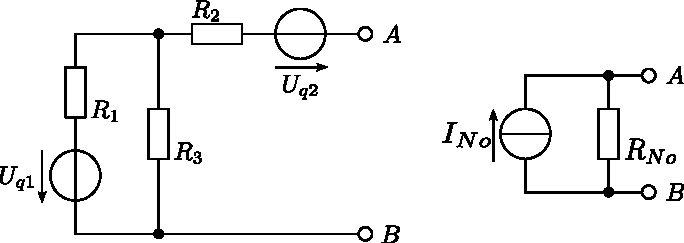
\includegraphics[scale=\schscale]{norton_sch_2.pdf}
\label{sch:norton}
\caption{Schaltung (l) und ihr Norton-Äquivalent (r)}
\end{figure}
    % Umwandlung Spannungsquelle <-> Stromquelle
% coding:utf-8

%----------------------------------------
%FOSAMATH, a LaTeX-Code for a mathematical summary for basic analysis
%Copyright (C) 2013, Daniel Winz, Ervin Mazlagic, Adrian Imboden, Philipp Langer

%This program is free software; you can redistribute it and/or
%modify it under the terms of the GNU General Public License
%as published by the Free Software Foundation; either version 2
%of the License, or (at your option) any later version.

%This program is distributed in the hope that it will be useful,
%but WITHOUT ANY WARRANTY; without even the implied warranty of
%MERCHANTABILITY or FITNESS FOR A PARTICULAR PURPOSE.  See the
%GNU General Public License for more details.
%----------------------------------------

% coding:utf-8
\section{Umwandlung Stern $\leftrightarrow$ Dreieck}
\begin{figure}[h!]
\centering
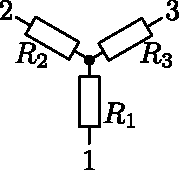
\includegraphics[width=0.30\textwidth]{star_sch.pdf}

\vspace{5mm}

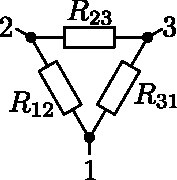
\includegraphics[width=0.30\textwidth]{tri_sch.pdf}
\label{sch:tristar}
\caption{Srern- und Dreieckschaltung}
\end{figure}

\subsection{Umwandlung Dreieck $\to$ Stern}
\[ \begin{matrix}
R_1 = \dfrac{R_{12} \cdot R_{31}}{R_{12} + R_{23} + R_{31}}\\\\
R_2 = \dfrac{R_{23} \cdot R_{12}}{R_{12} + R_{23} + R_{31}}\\\\
R_3 = \dfrac{R_{31} \cdot R_{23}}{R_{12} + R_{23} + R_{31}}\\\\
\end{matrix} \]

\subsection{Umwandlung Stern $\to$ Dreieck}
\[ \begin{matrix}
R_{12} = \dfrac{R_1 \cdot R_2 + R_2 \cdot R_3 + R_3 \cdot R_1}{R_3}\\\\
R_{23} = \dfrac{R_1 \cdot R_2 + R_2 \cdot R_3 + R_3 \cdot R_1}{R_1}\\\\
R_{31} = \dfrac{R_1 \cdot R_2 + R_2 \cdot R_3 + R_3 \cdot R_1}{R_2}\\\\
\end{matrix} \]     % Dreieck <-> Stern Umwandlung
% coding:utf-8

%FOSAET, a LaTeX-Code for a electrical summary of basic electronics
%Copyright (C) 2013, Daniel Winz, Ervin Mazlagic

%This program is free software; you can redistribute it and/or
%modify it under the terms of the GNU General Public License
%as published by the Free Software Foundation; either version 2
%of the License, or (at your option) any later version.

%This program is distributed in the hope that it will be useful,
%but WITHOUT ANY WARRANTY; without even the implied warranty of
%MERCHANTABILITY or FITNESS FOR A PARTICULAR PURPOSE.  See the
%GNU General Public License for more details.
%----------------------------------------

\section{Quellenverschiebung}     % Quellenverschiebung
% coding:utf-8

%FOSAET, a LaTeX-Code for a electrical summary of basic electronics
%Copyright (C) 2013, Daniel Winz, Ervin Mazlagic

%This program is free software; you can redistribute it and/or
%modify it under the terms of the GNU General Public License
%as published by the Free Software Foundation; either version 2
%of the License, or (at your option) any later version.

%This program is distributed in the hope that it will be useful,
%but WITHOUT ANY WARRANTY; without even the implied warranty of
%MERCHANTABILITY or FITNESS FOR A PARTICULAR PURPOSE.  See the
%GNU General Public License for more details.
%----------------------------------------

\section{Superposition}
Unter Superposition bzw. Überlagerung versteht man, dass gleiche Grössen sich linear überlagern.
In der Elektrotechnik z.B. bei der bestimmung von Netzwerkspannungen. 
So kann ein Netzwerk mit mehreren Quellen per Superposition einfach analysiert werden, indem man das Netzwerk mit jeweils einer aktiver Quelle betrachtet. 
Unabhängige Spannungsquellen werden kurzgeschlossen und unabhängige Stromquellen unterbrochen.
Die Ergenisse jeder Betrachtung können dann linear kombiniert bzw. überlagert werden.
    % Superposition bzw. Überlagerung
% coding:utf-8

%FOSAET, a LaTeX-Code for a electrical summary of basic electronics
%Copyright (C) 2013, Daniel Winz, Ervin Mazlagic

%This program is free software; you can redistribute it and/or
%modify it under the terms of the GNU General Public License
%as published by the Free Software Foundation; either version 2
%of the License, or (at your option) any later version.

%This program is distributed in the hope that it will be useful,
%but WITHOUT ANY WARRANTY; without even the implied warranty of
%MERCHANTABILITY or FITNESS FOR A PARTICULAR PURPOSE.  See the
%GNU General Public License for more details.
%----------------------------------------

\newpage
\section{Knotenpotentialverfahren}
\begin{enumerate}
  \item Alle realen Spannungsquellen in Stromquellen umwandeln. 
  \item Null-Potential ($N_0$) wählen (bestenfalls dort wo der Strom gesucht ist)
  \item restliche Knoten nummerieren ($N_1$, $N_2$, $N_3$ ...$N_n$)
  \item Matrix aufstellen
  \item Links alle Knoten ohne den Bezugsknoten auflisten
  \item Oben alle Spannungen von den Knoten zum Bezugsknoten eintragen
  \item Hauptdiagonale ausfüllen: \\
  Dazu sind die Leitwerte aller Widerstände, die am jeweiligen Knoten angeschlossen sind zu addieren und hinzuschreiben. 
  \item Restliche Matrix ausfüllen: \\
  Dazu sind die Leitwerte aller Widerstände, die direkt zwischen den jeweiligen Knoten liegen zu addieren und einzutragen. Das Vorzeichen ist dabei immer negativ. Die Hauptachse bildet dabei eine Symmetrieachse. \\
  Liegt keine direkte Verbindung zwischen zwei Knoten, so wird 0 eingetragen
  \item In der rechten Spalte Stromquellen eintragen. \\
  Das Vorzeichen ist dabei abhängig von der Flussrichtung: \\
  \begin{itemize}
    \item[+] wenn der Strom in den Knoten fliesst
    \item[-] wenn der Strom vom Knoten weg fliesst
  \end{itemize}
\end{enumerate}

\newpage
\subsection{Beispiel}

\begin{figure}[h!]
\centering
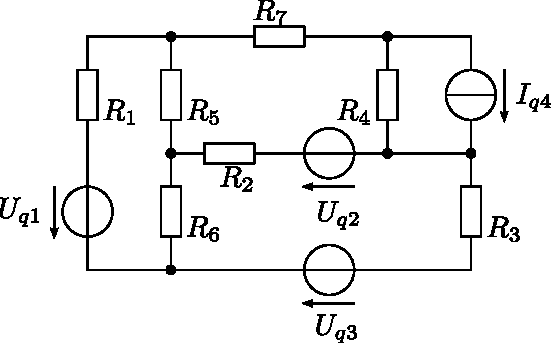
\includegraphics[scale=\schscale]{knotpot_sch.pdf}
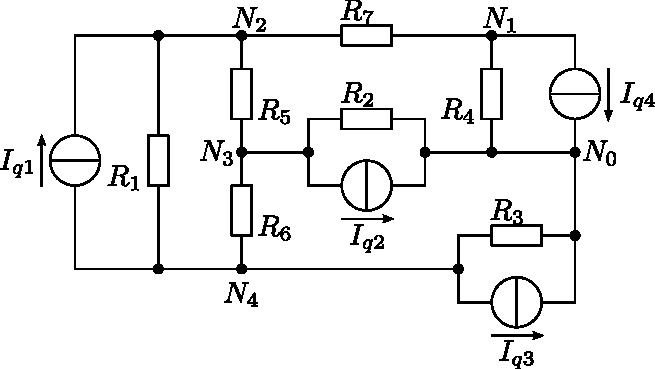
\includegraphics[scale=\schscale]{knotpot_sch_2.pdf}
\caption{Umwandlung von Strom- zu Spannungsquellen}
\label{sch:knotpot_2}
\end{figure}

\begin{table}[h!]
\footnotesize
\[ 	\begin{array}{c|cccc||c}
	N & U_{10}						& U_{20}										& U_{30} 											& U_{40} 											& I \\
	\hline &&&&& \\
	N_1	& \frac{1}{R_4} + \frac{1}{R_7}		& -\frac{1}{R_7} 								& 0 												& 0 												& -I_{q4} 			\\
	&&&&& \\
	N_2	& -\frac{1}{R_7} 					& \frac{1}{R_1} + \frac{1}{R_5} + \frac{1}{7} 	& -\frac{1}{R_5} 									& -\frac{1}{R_1} 									& I_{q1} 			\\ 
	&&&&& \\
	N_3	& 0 								& -\frac{1}{R_5} 								& \frac{1}{R_2} + \frac{1}{R_5} + \frac{1}{R_6} 	& -\frac{1}{R_6} 									& -I_{q2} 			\\ 
	&&&&& \\
	N_4 & 0 								& -\frac{1}{R_1} 								& -\frac{1}{R_6} 									& \frac{1}{R_1} + \frac{1}{R_3} + \frac{1}{R_6} 	& -I_{q2} -I_{q3} 	\\ 
	&&&&& \\
	\end{array}
\]
\normalsize
\caption{Matrix zu Abb.~\ref{sch:knotpot_2}}
\end{table}

\newpage
     % Knotenpotentialverfahren
% coding:utf-8

%----------------------------------------
%FOSAMATH, a LaTeX-Code for a mathematical summary for basic analysis
%Copyright (C) 2013, Daniel Winz, Ervin Mazlagic, Adrian Imboden, Philipp Langer

%This program is free software; you can redistribute it and/or
%modify it under the terms of the GNU General Public License
%as published by the Free Software Foundation; either version 2
%of the License, or (at your option) any later version.

%This program is distributed in the hope that it will be useful,
%but WITHOUT ANY WARRANTY; without even the implied warranty of
%MERCHANTABILITY or FITNESS FOR A PARTICULAR PURPOSE.  See the
%GNU General Public License for more details.
%----------------------------------------

% coding:utf-8
\section{Maschenstromverfahren}

\begin{itemize}
	\item Alle realen Quellen in Spannungsquellen wandeln
	\item Maschen legen und nummerieren ($M_1$, $M_2$, $M_3$ ...$M_n$)
	\item Baum bilden (Baum bedeutet hier ein Strang, welcher alle Knoten berührt und durchgehend verbunden ist. Dieser muss keine \textit{Schlange} darstellen, sondern darf auch sternförmig etc. sein.
	\item Matrix aufstellen
	\item Links alle Maschen auflisten
	\item Oben alle Ströme der Quellen eintragen welche zwischen Knoten liegen (nicht jener die innerhalb des Baumes liegen)
	\item Hauptdiagonale ausfüllen:\\ Hierzu sind alle Widerstandswerte zu summieren welche in entsprechender Masche liegen.
	\item Restliche Matrix ausfüllen:\\ Hierzu sind alle Widerstandswerte einzutragen welche zu zwei Maschen gehören einzutragen. Das Vorzeichen ist positiv zu wählen, falls die Maschenpfeilrichtung die selbe ist, sonst negativ.
	\item In der rechten Spalte Spannungsquellen eintragen. Das Vorzeichen ist dabei positiv, falls die Maschenpfeilrichtung entgegen der Spannungspfeilrichtung ist, sonst negativ.
\end{itemize}

\newpage

\subsection{Beispiel}
\begin{figure}[h!]
\centering
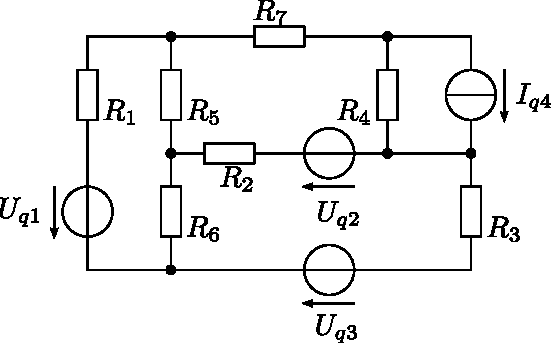
\includegraphics[width=0.55\textwidth]{mastro_sch.pdf}

\vspace{5mm}

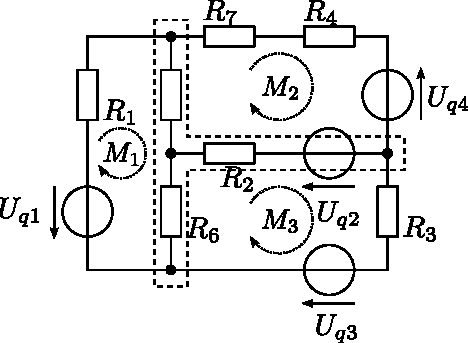
\includegraphics[width=0.50\textwidth]{mastro_sch_2.pdf}
\label{sch:mastro}
\caption{Schaltung zum Maschenstromverfahren}
\end{figure}

\begin{figure}[h!]
\footnotesize
\[ \begin{array}{c|ccc||c}

M	& I_1 & I_4 & I_3 & U \\
\hline &&&& \\
M_1 	& R_1 + R_2 + R_3 	& -R_5 				& -R_6 			& U_{q1} \\
&&&& \\
M_2 	& -R_5 			& R_2 + R_4 + R_5 + R_7 	& -R_2 			& U_{q4} \\
&&&& \\
M_3 	& -R_6 			& -R_2 				& R_2 + R_3 + R_6 	& -U_{q3} \\
\end{array}
\]
\normalsize
\caption{Matrix zu Abb.~\ref{sch:mastro}}
\end{figure}
      % Maschenstromverfahren
